\normaltrue \difficilefalse \tdifficilefalse
\correctiontrue

%\UPSTIidClasse{11} % 11 sup, 12 spé
%\newcommand{\UPSTIidClasse}{12}
% CCP MP 2016
\exer{Robot de maraîchage Oz 440 $\star$ \label{A3:01:58}}
\setcounter{numques}{0}
\UPSTIcompetence[2]{A3-01}
\index{Compétence A3-01}
\index{Robot de maraîchage Oz 440 }
\index{Associer les fonctions aux constituants.}

\ifcorrection
\else
\textbf{Pas de corrigé pour cet exercice.}
\fi

\ifprof
\else

Le robot de maraîchage Oz 440 développé par la société Naïo Technologies est un outil autonome
agricole, alliant robustesse et écologie, capable d’assister les maraîchers dans les tâches les plus
pénibles comme le transport de charges lors des récoltes et le désherbage mécanique à l’aide d’un
outil de binage.


\begin{figure}[H]
\centering
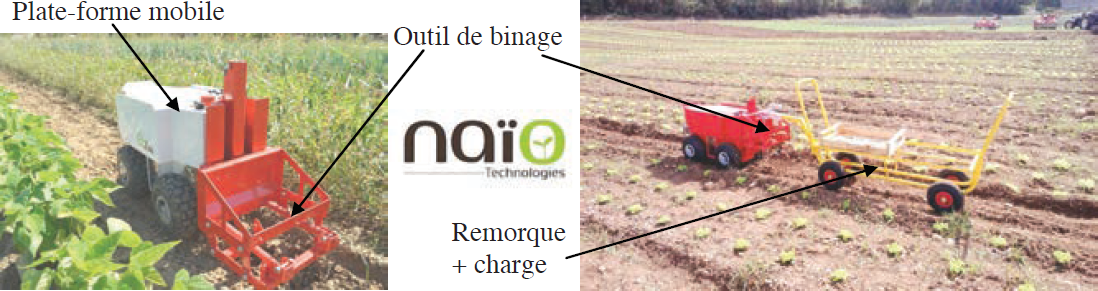
\includegraphics[width=\linewidth]{58_01}
%\caption{Amplificateur de charge à plusieurs canaux KISTLER. \label{fig_50_01}}
\end{figure}


Ce robot est constitué d’une plate-forme mobile électrique à 4 roues motrices sur laquelle sont
fixés divers outils et capteurs. La figure 1 donne la structure du robot sous la forme d’un
diagramme de définition de blocs (BDD) avec les propriétés principales de chaque constituant,
utiles pour la résolution du problème.

\begin{figure}[H]
\centering
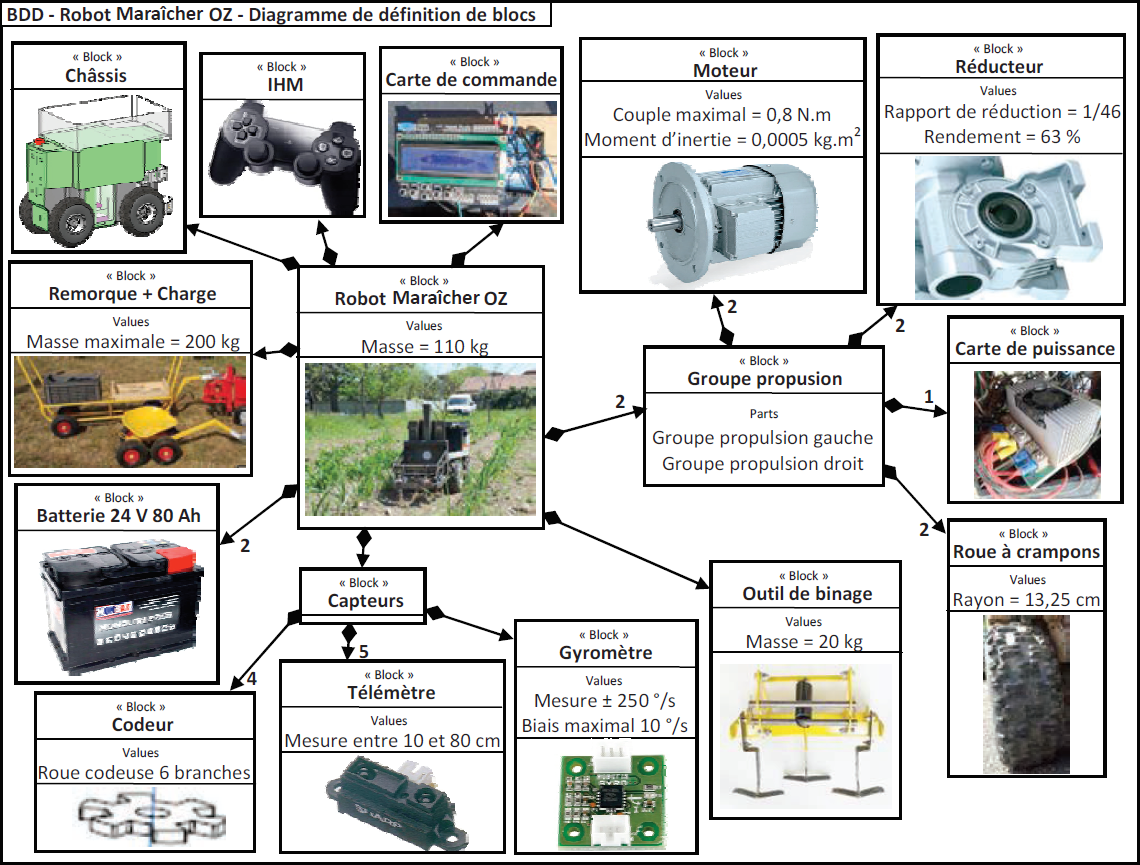
\includegraphics[width=\linewidth]{58_02}
%\caption{Amplificateur de charge à plusieurs canaux KISTLER. \label{fig_50_01}}
\end{figure}


Ce robot de petite taille évolue directement entre les rangées de cultures pour un travail de
précision. Il peut, par exemple, désherber et aussi suivre des personnes lors de la récolte tout en
transportant des charges. Bien plus petit qu’un tracteur classique, il ne casse pas la structure
naturelle du sol et évite ainsi le phénomène de compaction des sols provoqué habituellement par les
tracteurs ou le piétinement de l’homme. Il roule lentement et passe au plus près des cultures sans
risquer de les abîmer. Selon le vieil adage « un binage vaut deux arrosages », le fait de pouvoir
utiliser ce robot régulièrement, sans perte de temps, permet de toujours avoir un sol parfaitement
biné et ainsi de diminuer les effets d’évaporation de l’eau.
\fi

\question{À l’aide du diagramme de définition de blocs disponible, réaliser le diagramme correspondant à la chaîne fonctionnelle de l’ensemble
groupe propulsion droit du robot.}
\ifprof

\begin{figure}[H]
\centering
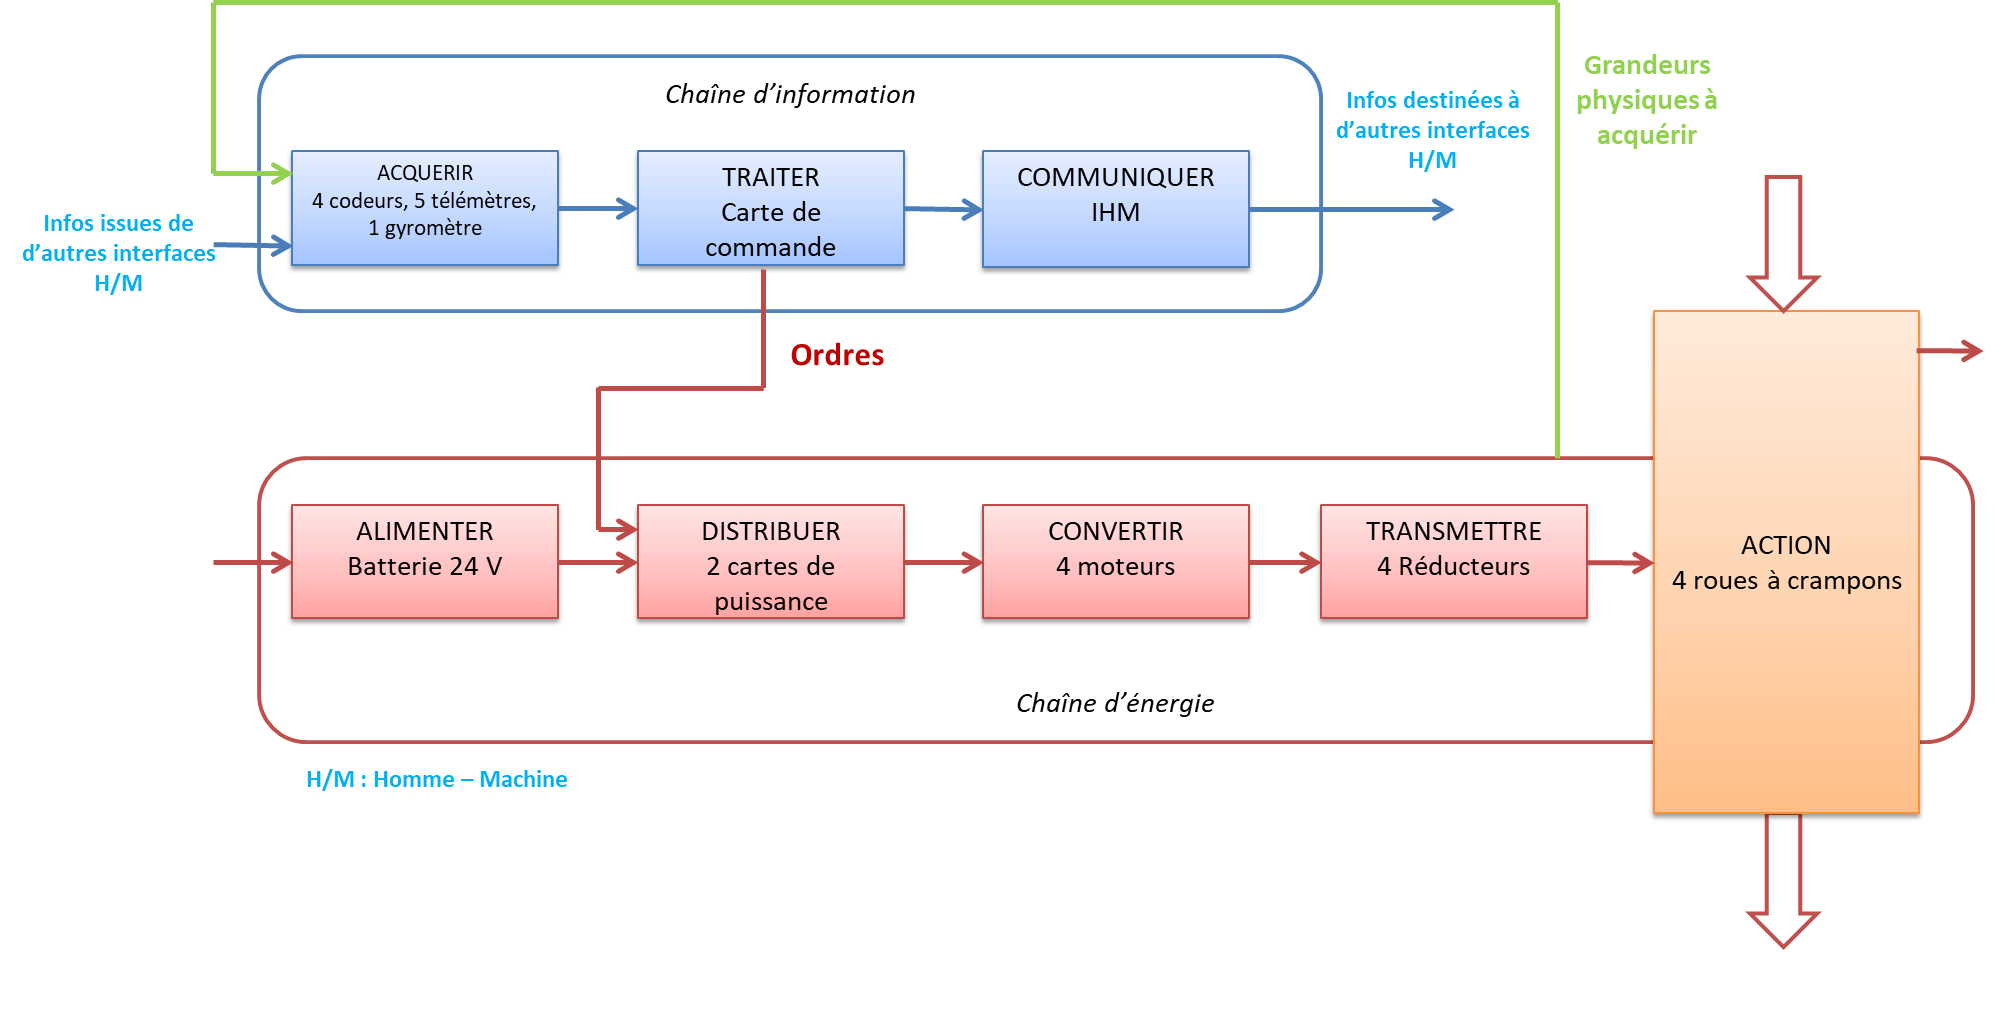
\includegraphics[width=\linewidth]{58_01_cor}
%\caption{Amplificateur de charge à plusieurs canaux KISTLER. \label{fig_50_01}}
\end{figure}

\else
\begin{flushright}
\footnotesize{Corrigé  voir \ref{A3:01:58}.}
\end{flushright}%
\fi